\documentclass{beamer}

\usetheme{Madrid}
\usepackage{tikz}
\usetikzlibrary{positioning}
\usepackage{graphicx}
% \usepackage{enumitem}


\title{\textcolor{red} {\textbf{Red}}-\textcolor{black}{\textbf{Black}} \textbf{Tree}}
%\subtitle{This is a subtitle}
\author[Souvik \and Sagor \and Kausar]
{\textbf{\small{Souvik Mondol - 2005069}} \\
\textbf{\small{Sagor Chanda - 2005071}} \\
\textbf{\small{S.M Kausar Parvej - 2005076}}
}

\institute[CSE, BUET]
{
	Department of CSE\\
	Bangladesh University of Engineering and Technology
}
\date{\small{\today}}

% \AtBeginSection
% {
% 	\begin{frame}
% 		\frametitle{Contents}
% 		\tableofcontents[currentsection]
% 	\end{frame}
% }




\begin{document}
\frame{\titlepage}

\begin{frame}
		\frametitle{Objectives}
		\tableofcontents
\end{frame}

\section*{Figure}
\begin{frame}{Figure}
			\begin{figure}
				\centering
				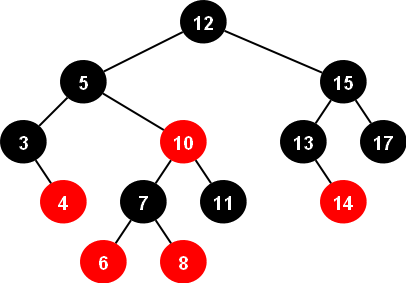
\includegraphics[scale=0.4]{redblacktree.png}
				\caption{A Image of \textcolor{red} {\textbf{Red}}-\textbf{black} Tree}
			\end{figure}
		\end{frame}

\begin{frame}{\textcolor{red} {\textbf{Red}}-\textcolor{black}{\textbf{Black}} Tree}
\begin{center}
    \huge{What is a \textcolor{red}{Red}-Black tree?}
\end{center}
    
\end{frame}





\section{Introduction}
\begin{frame}{What is \textcolor{red} {\textbf{Red}}-\textcolor{black}{\textbf{Black}} Tree?}
    \begin{block}{Definition of Red-Black Tree}
    Red-Black tree is a \textcolor{red}{\textbf{Binary Search Tree}} in which every node is colored with either red or black.
\end{block}

\begin{block}{}
	It is a type of self balancing binary search tree.It has a good efficient worst case running time complexity.
			\end{block}
\end{frame}



\section{Define the red-black tree properties }
\begin{frame}{Binary Search Trees - Performance}


{\begin{itemize}
    \item  Insertion and removal from 
BSTs is O(height)
\item What is the height of a 
BST?
\begin{itemize}
    \item  If the tree is balanced: 
O(logn)
\item  If the tree is very 
unbalanced: O(n)
\end{itemize}
\end{itemize}}


    \centering

\begin{table}
    \centering
    \begin{tabular}{cc}
        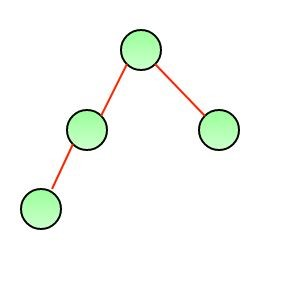
\includegraphics[scale=0.4]{tree11.jpg} & 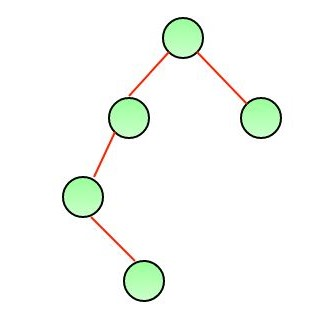
\includegraphics[scale=0.4]{tree22.jpg}\\
        Balanced  BST & Unbalanced BST\\
    \end{tabular}
    
    \label{tab:my_label}
\end{table}
    
\end{frame}

\section*{Balanced BSTs}
\begin{frame}{Balanced BSTs}
    \begin{itemize}
        \item Define a balanced binary tree as one where
        \begin{itemize}
            \item  There is no path from the root to a leaf that is more than 
twice as long as any other such path
\item The height of such a tree is O(logn)
        \end{itemize}

        \item Guaranteeing that a BST is balanced requires either
        \begin{itemize}
            \item  A more complex structure (2-3 and 2-3-4 trees) or
            \item  More complex insertion and deletion algorithms (red
black trees)
        \end{itemize}
    \end{itemize}
\end{frame}


%page red black tree structrue

\section*{red black tree structrue}
\begin{frame}{\textcolor{red} {\textbf{Red}}-\textcolor{black}{\textbf{Black}} Tree Structures}
    \begin{itemize}
        \item A red-black tree is a balanced BST
        \item Each node has an extra colour field which is
        \begin{itemize}
            \item \textcolor{red}{\textbf{Red}}- \textbf{Black}
            \begin{itemize}
                \item  Usually represented as a boolean– \textbf{isBlack}
            \end{itemize}
        \end{itemize}
        \item Nodes have an additional pointer to their parent
        \item  A node’s null child pointers are treated as if they 
were black nodes
\begin{itemize}
    \item These null children are imaginary nodes so are not 
allocated space
\item And are always coloured black
\end{itemize}
    \end{itemize}
\end{frame}

%red black tree nodes
\section*{red black tree nodes}
\begin{frame}{\textcolor{red} {\textbf{Red}}-\textcolor{black}{\textbf{Black}} tree nodes}
    \begin{itemize}
    \item  Red-black trees are reference structures
    \item Nodes contain data, three pointers to nodes, and 
the node’s colour
\end{itemize}


\end{frame}



%red black tree properties
\section*{red black Tree Properties}
\begin{frame}{\textcolor{red} {\textbf{Red}}-\textcolor{black}{\textbf{Black}} tree properties}

\begin{enumerate}
\item  Every node is either \textcolor{red} {red} or\textbf{ black}
\item Every leaf is \textbf{black}
\begin{itemize}
    \item  Leaves refers to the imaginary nodes
    \begin{itemize}
        \item i.e. every null child of a node is considered to be a black leaf
    \end{itemize}
\end{itemize}
\item If a node is \textcolor{red} {red} both its children must be \textbf{black}
\item Every path from a node to a leaf contains the same 
number of black nodes
\item  The root is \textbf{black}-for convenience
\end{enumerate}
    
\end{frame}

%Red black tree height
\section*{Red black tree height}
\begin{frame}{\textcolor{red} {\textbf{Red}}-\textcolor{black}{\textbf{Black}} Tree Height}
\begin{itemize}
    \item The black height of a node, bh(v), is the number of black 
nodes on a path from v to a null black child
\begin{itemize}
    \item  Without counting v itself
    \item  Property 4–every path from a node to a leaf contains the same 
number of black nodes

\end{itemize}
\item  The height of a node, h(v), is the number of nodes on 
the longest path from v to a leaf
\begin{itemize}
    \item  Without counting v itself
    \item Property 3– a red node’s children must be black
    \begin{itemize}
        \item So $ h(v) <=2(bh(v))$
    \end{itemize}
\end{itemize}
\end{itemize}
    
\end{frame}

%Balanced trees
\section*{Balanced trees}
\begin{frame}{Balanced Trees}

\begin{itemize}
    \item It can be shown that a tree with the red-black structure is balanced.
    \item A balanced tree has no path from the root to a leaf that is more than twice as long as any other such path.
    \item Assume that a tree has \( n \) internal nodes:
    \begin{itemize}
        \item An internal node is a non-leaf node, and the leaf nodes are imaginary nodes, so \( n \) is the number of actual nodes.
        \item A red-black tree has \(\geq 2bh - 1\) internal (real) nodes.
        \begin{itemize}
        
        \item Can be proven by induction (e.g., Algorithms, Cormen et al).
        \item But consider that a perfect tree has \(2^h+1\) leaves, \(bh\) must be less than or equal to \(h\), and that \(2^h+1 = 2^h + 2^h\).
        \end{itemize}
    \end{itemize}
\end{itemize}

  
\end{frame}


%REd black tree height
\section*{red black tree height}
\begin{frame}{\textcolor{red} {\textbf{Red}}-\textcolor{black}{\textbf{Black}} Tree Height}

\begin{itemize}
    \item Claim: A red-black tree has height, \( h \leq 2 \cdot \log(n+1) \).
    \begin{enumerate}
        \item \( n \geq 2bh - 1 \) from claim on the previous slide.
        \item \( bh \geq h/2 \) (red nodes must have black children).
        \item \( n \geq 2h/2 - 1 \) (replace \( bh \) in 1 with \( h \)).
        \item \( \log(n+1) \geq h/2 \) (take logarithm base 2 of both sides of 3, and add 1).
        \item \( 2 \cdot \log(n+1) \geq h \) (multiply both sides of 4 by 2).
        \item \( h \leq 2 \cdot \log(n+1) \) (reverse 5).
    \end{enumerate}
    \item Note that \( 2 \cdot \log(n+1) \) is \( O(\log(n)) \).
    \begin{itemize}
        \item If insertion and removal are \( O(\text{height}) \), they are \( O(\log(n)) \).
    \end{itemize}
\end{itemize}
    
\end{frame}

%rotations
\section{Rotations}
\begin{frame}{\textcolor{red} {\textbf{Red}}-\textcolor{black}{\textbf{Black}} Tree : Rotation}
    \begin{center}
        {\Huge\textbf{\textcolor{blue}{Rotation}}}
    \end{center}
\end{frame}



\section*{Rotations}
\begin{frame}{Rotations}

    \begin{itemize}
    \item An item must be inserted into a red-black tree at the correct position.
    \item The shape of a tree is determined by:
    \begin{itemize}
        \item The values of the items inserted into the tree.
        \item The order in which those values are inserted.
    \end{itemize}
    \item This suggests that there is more than one tree (shape) that can contain the same values.
    \item A tree's shape can be altered by rotation while still preserving the binary search tree (BST) property.
\end{itemize}
\end{frame}


%left rotation
\section*{Left rotation}
\begin{frame}{Left Rotation}
\begin{block}{Left Rotation}
    In left-rotation, the arrangement of the nodes on the right is transformed into the arrangements on the left node.
\end{block}
    \textcolor{blue}{\textbf{Let the initial tree be: }}
    \begin{figure}[h]
        \centering
        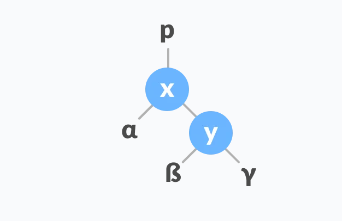
\includegraphics[scale=0.8]{rotation_Images/Screenshot 2024-02-19 224631.png}
    \caption{Initial Tree}
    \end{figure}  
\end{frame}



\begin{frame}{Left Rotation}
    \begin{itemize}
        \item If y has a left subtree, assign x as the parent of the left subtree of y.
    \end{itemize}
    \begin{figure}[h]
        \centering
        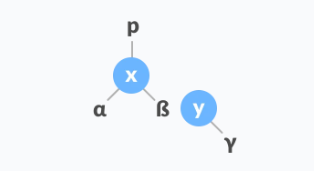
\includegraphics[scale=0.8]{rotation_Images/Screenshot 2024-02-19 224935.png}
    \caption{Assign x as the parent of the left subtree of y}
    \end{figure} 
\end{frame}



\begin{frame}{Left Rotation}
    \begin{itemize}
        \item If the parent of x is NULL, make y as the root of the tree.
        \item Else if x is the left child of p, make y as the left child of p.
        \item Else assign y as the right child of p.
    \end{itemize}

    \begin{figure}
        \centering
        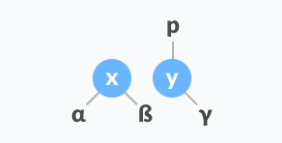
\includegraphics{rotation_Images/Screenshot 2024-02-19 230725.png}
        \caption{Change the parent of x to that of y}
        
    \end{figure}
\end{frame}

\begin{frame}{Left Rotation}
    \begin{itemize}
        \item Make y as the parent of x.
    \end{itemize}
    \begin{figure}
        \centering
        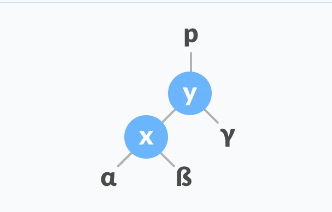
\includegraphics{rotation_Images/Screenshot 2024-02-19 231056.png}
        \caption{Assign y as the parent of x.}
        \label{fig:enter-label}
    \end{figure}
\end{frame}


\begin{frame}{Right Rotation}
\begin{block}{Right Rotate}
    In right-rotation, the arrangement of the nodes on the left is transformed into the arrangements on the right node.
\end{block}
\textcolor{blue}{\textbf{Let the initial tree be: }}
    \begin{figure}[h]
        \centering
        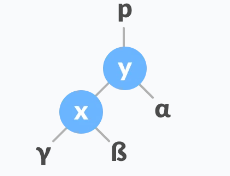
\includegraphics[scale=0.8]{rotation_Images/Screenshot 2024-02-19 231255.png}
    \caption{Initital Tree}
    \end{figure}  
\end{frame}


\begin{frame}{Right Rotate}
    \begin{itemize}
        \item If x has a right subtree, assign y as the parent of the right subtree of x.
    \end{itemize}
    \begin{figure}
        \centering
        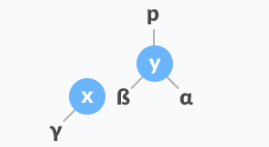
\includegraphics{rotation_Images/Screenshot 2024-02-19 231509.png}
        \caption{Assign y as the parent of the right subtree of x}
        \label{fig:enter-label}
    \end{figure}
\end{frame}

\begin{frame}{Right Rotate}
    \begin{itemize}
        \item If the parent of y is NULL, make x as the root of the tree.
        \item Else if y is the right child of its parent p, make x as the right child of p.
        \item Else assign x as the left child of p.
    \end{itemize}
    \begin{figure}
        \centering
        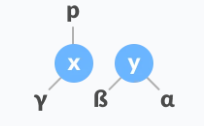
\includegraphics{rotation_Images/Screenshot 2024-02-19 231754.png}
        \caption{Assign the parent of y as the parent of x}
        \label{fig:enter-label}
    \end{figure}
\end{frame}

\begin{frame}{Right Rotate}
    \begin{itemize}
        \item Make x as the parent of y.
    \end{itemize}
    \begin{figure}
        \centering
        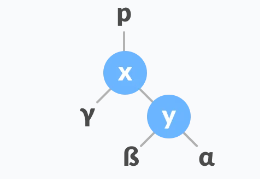
\includegraphics{rotation_Images/Screenshot 2024-02-19 231909.png}
        \caption{Assign x as the parent of y}
        \label{fig:enter-label}
    \end{figure}
\end{frame}



\begin{frame}{Left-Right Rotate}
    \begin{block}{Left-Right Rotate}
     In left-right rotation, the arrangements are first shifted to the left and then to the right.   \end{block}
     \begin{itemize}
         \item Do left rotation on x-y.
     \end{itemize}
     \begin{figure}
         \centering
         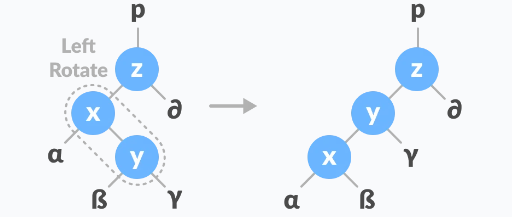
\includegraphics{rotation_Images/Screenshot 2024-02-19 232205.png}
         \caption{Left rotate x-y}
         \label{fig:enter-label}
     \end{figure}
\end{frame}


\begin{frame}{Left-Right Rotate}
    \begin{itemize}
        \item Do right rotation on y-z.
    \end{itemize}
    \begin{figure}
        \centering
        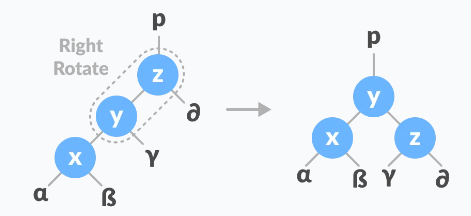
\includegraphics{rotation_Images/Screenshot 2024-02-19 232348.png}
        \caption{Right rotate z-y}
        \label{fig:enter-label}
    \end{figure}
\end{frame}


\begin{frame}{Right-Left Rotate}
    \begin{block}{Right-Left Rotate}
        In right-left rotation, the arrangements are first shifted to the right and then to the left.
    \end{block}
    \begin{itemize}
        \item Do right rotation on x-y.
    \end{itemize}
    \begin{figure}
        \centering
        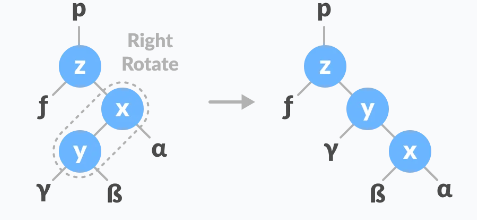
\includegraphics{rotation_Images/Screenshot 2024-02-19 232917.png}
        \caption{Right rotate x-y}
        \label{fig:enter-label}
    \end{figure}
\end{frame}


\begin{frame}{Right-Left}
    \begin{itemize}
        \item Do left rotation on z-y.
    \end{itemize}
    \begin{figure}
        \centering
        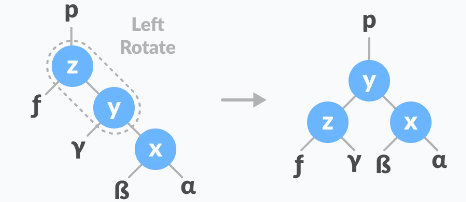
\includegraphics{rotation_Images/Screenshot 2024-02-19 233032.png}
        \caption{Left rotate z-y}
        \label{fig:enter-label}
    \end{figure}
\end{frame}










%Insertion 
\section{Insertion}
\begin{frame}{Red-Black Trees}
    \begin{center}
        {\Huge\textbf{\textcolor{blue}{Insertion}}}
    \end{center}
\end{frame}

\begin{frame}{Red-Black Tree Insertion Steps}
\begin{itemize}
    \item[\textbullet] \textbf{Insert as for a BST and make the new node red}
    \begin{itemize}
        \item The only property that can be violated is that both a red node’s children are black (its parent may be red)
    \end{itemize}
    \item[\textbullet] \textbf{If this is the case, try to fix it by coloring the new node red and making its parent and uncle black}
    \begin{itemize}
        \item Which only works if both were red
        \item As otherwise the equal black height property will be violated
    \end{itemize}
    \item[\textbullet] \textbf{If changing the colors doesn’t work, the tree must be rotated}
    \begin{itemize}
        \item Which also entails changing some colors
    \end{itemize}
\end{itemize}
\end{frame}


\begin{frame}{Red-Black Tree Insertion Simulation}
\textbf{Step 1: Insert as for a BST and make the new node red \\(Inserting 4)}
\begin{center}
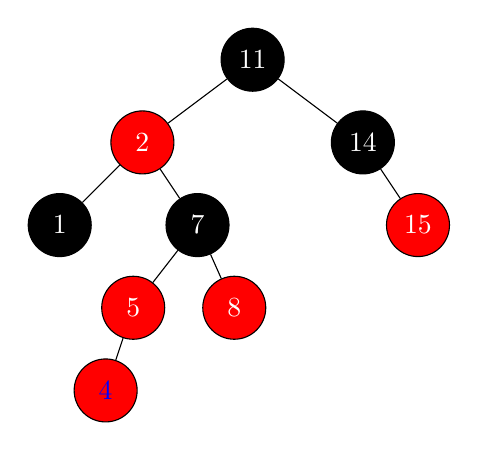
\begin{tikzpicture}[scale=0.7,level/.style={sibling distance=40mm/#1}]
\tikzstyle{every node}=[circle,draw,minimum size=8mm]
\node[fill=black,text=white] (a) {11}
  child {node[fill=red,text=white] (b) {2}
    child [xshift=-0.5cm] {node[fill=black,text=white] {1}}
    child {node[fill=black,text=white] {7}
        child[xshift=-0.5cm] {node[fill=red,text=white] {5}
            child[xshift=-0.5cm] {node[fill=red,text=blue] {4}}
        }
        child {node[fill=red,text=white] {8}}
    }
  }
  child {node[fill=black,text=white] (c) {14}
    child [xshift=1cm] {node[fill=red,text=white] {15}}
  };
\end{tikzpicture}
\end{center}
\end{frame}

\begin{frame}{Red-Black Tree Insertion Simulation}
\textbf{Step 2: 4, it's parent 5 and uncle 8 all are red \\ (So making 5, 7 and 8 inverting their color)}
\begin{center}
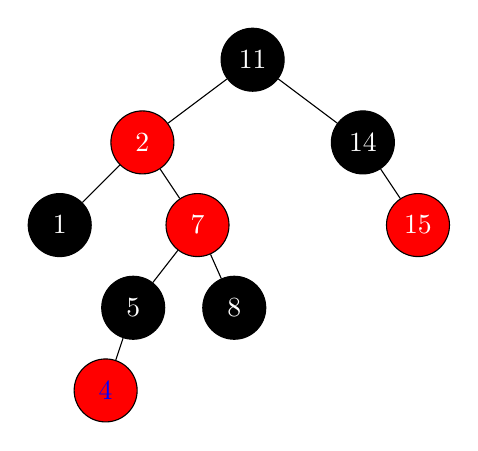
\begin{tikzpicture}[scale=0.7,level/.style={sibling distance=40mm/#1}]
\tikzstyle{every node}=[circle,draw,minimum size=8mm]
\node[fill=black,text=white] (a) {11}
  child {node[fill=red,text=white] (b) {2}
    child [xshift=-0.5cm] {node[fill=black,text=white] {1}}
    child {node[fill=red,text=white](c) {7}
        child[xshift=-0.5cm] {node[fill=black,text=white] {5}
            child[xshift=-0.5cm] {node[fill=red,text=blue] {4}}
        }
        child {node[fill=black,text=white] {8}}
    }
  }
  child {node[fill=black,text=white]  {14}
    child [xshift=1cm] {node[fill=red,text=white] {15}}
  };
\end{tikzpicture}
\end{center}
\end{frame}

\begin{frame}{Red-Black Tree Insertion Simulation}
\textbf{Step 3: Now 7 and it's parent 2 are both red but 7's uncle 14 is black (So Left rotating 2)}
\begin{center}
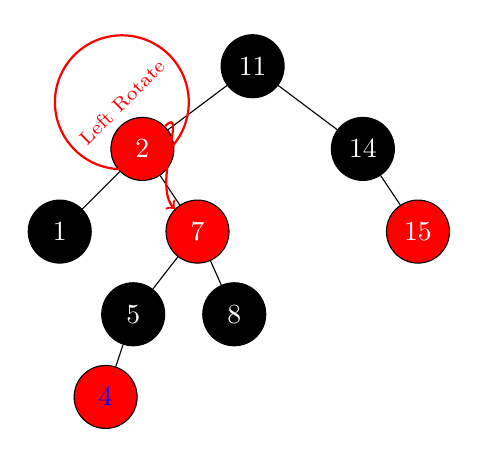
\begin{tikzpicture}[scale=0.7,level/.style={sibling distance=40mm/#1}]
\tikzstyle{every node}=[circle,draw,minimum size=8mm]
\node[fill=black,text=white] (a) {11}
  child {node[fill=red,text=white] (b) {2}
    child [xshift=-0.5cm] {node[fill=black,text=white] {1}}
    child {node[fill=red,text=white](c) {7}
        child[xshift=-0.5cm] {node[fill=black,text=white] {5}
            child[xshift=-0.5cm] {node[fill=red,text=blue] {4}}
        }
        child {node[fill=black,text=white] {8}}
    }
  }
  child {node[fill=black,text=white]  {14}
    child [xshift=1cm] {node[fill=red,text=white] {15}}
  };
  \draw[->,red,thick] (b) to[out=45,in=135] node[above,rotate=45,font=\scriptsize] {Left Rotate} (c);
\end{tikzpicture}
\end{center}
\end{frame}

\begin{frame}{Red-Black Tree Insertion Simulation}
\begin{center}
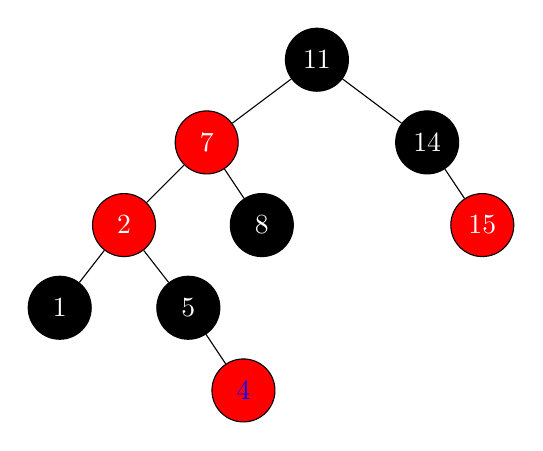
\begin{tikzpicture}[scale=0.7,level/.style={sibling distance=40mm/#1}]
\tikzstyle{every node}=[circle,draw,minimum size=8mm]
\node[fill=black,text=white] (a) {11}
  child {node[fill=red,text=white] (b) {7}
    child [xshift=-0.5cm] {node[fill=red,text=white] {2}
        child [xshift=-0.5cm] {node[fill=black,text=white] {1}}
        child[xshift=0.5cm] {node[fill=black,text=white] {5}
            child[xshift=1cm] {node[fill=red,text=blue] {4}}
        }
    }
    child {node[fill=black,text=white] {8}}
  }
  child {node[fill=black,text=white] (c) {14}
    child [xshift=1cm] {node[fill=red,text=white] {15}}
  };
\end{tikzpicture}
\end{center}
\end{frame}

\begin{frame}{Red-Black Tree Insertion Simulation}
\textbf{Step 4: Now 2 and it's parent 2 are both red but 2's uncle 14 is black and  2 is a left child\\(So inverting the color of 7 \& 11 and right rotating 11)}
\begin{center}
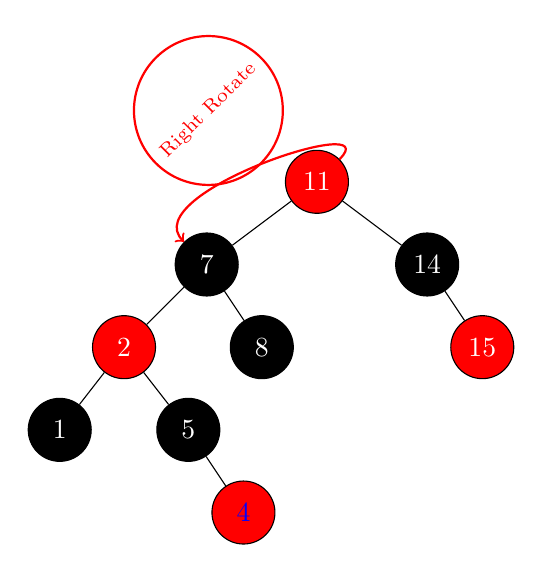
\begin{tikzpicture}[scale=0.7,level/.style={sibling distance=40mm/#1}]
\tikzstyle{every node}=[circle,draw,minimum size=8mm]
\node[fill=red,text=white] (a) {11}
  child {node[fill=black,text=white] (b) {7}
    child [xshift=-0.5cm] {node[fill=red,text=white] {2}
        child [xshift=-0.5cm] {node[fill=black,text=white] {1}}
        child[xshift=0.5cm] {node[fill=black,text=white] {5}
            child[xshift=1cm] {node[fill=red,text=blue] {4}}
        }
    }
    child {node[fill=black,text=white] {8}}
  }
  child {node[fill=black,text=white] (c) {14}
    child [xshift=1cm] {node[fill=red,text=white] {15}}
  };
  \draw[->,red,thick] (a) to[out=45,in=135] node[above,rotate=45,font=\scriptsize] {Right Rotate} (b);
\end{tikzpicture}
\end{center}
\end{frame}

\begin{frame}{Red-Black Tree Insertion Simulation}
\textbf{And here the balanced Tree!!}
\begin{center}
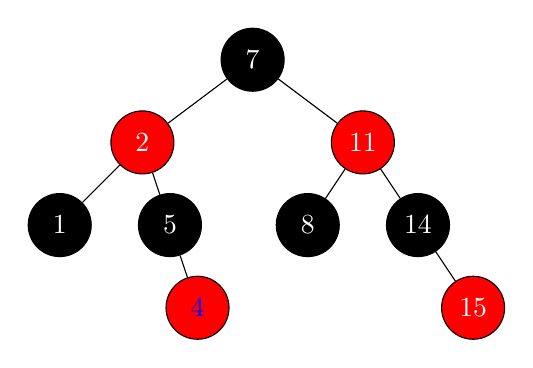
\begin{tikzpicture}[scale=0.7,level/.style={sibling distance=40mm/#1}]
\tikzstyle{every node}=[circle,draw,minimum size=8mm]
\node[fill=black,text=white] (a) {7}
  child {node[fill=red,text=white] (b) {2}
    child [xshift=-0.5cm] {node[fill=black,text=white] {1}}
    child [xshift=-0.5cm] {node[fill=black,text=white] {5}
        child[xshift=0.5cm] {node[fill=red,text=blue] {4}}
    }
  }
    child {node[fill=red,text=white] {11}
        child {node[fill=black,text=white] (c) {8}}
        child {node[fill=black,text=white] (c) {14}
        child [xshift=1cm] {node[fill=red,text=white] {15}}
    }
  };
\end{tikzpicture}
\end{center}
\end{frame}






% Souvik's Part starts...
\section{Deletion}
\begin{frame}{Red-Black Trees}
    \begin{center}
        {\Huge\textbf{\textcolor{blue}{Deletion}}}
    \end{center}
\end{frame}

\begin{frame}{Red-Black Trees: Deletion}
    \begin{itemize}
        \item  Deletion, like insertion, should preserve all the Red-Black properties.        
        \item \vspace{0.2cm} Steps of deletion:
        \vspace{0.1cm}
        \begin{itemize}
            \item[$\blacksquare$]  Do regular BST deletion.
            \item[$\blacksquare$]  Fix any violations of Red-Black properties that may result.
        \end{itemize}
    \end{itemize}
\end{frame}

\begin{frame}{Red-Black Trees: Deletion}
        Deletion is a fairly complex process. Before going through the steps, one must know about \textbf{\textit{double black}}. \\
\end{frame}

\begin{frame}{Red-Black Trees: Deletion}
        Deletion is a fairly complex process. Before going through the steps, one must know about \textbf{\textit{double black}}. \\

        \vspace{0.5cm}
        \begin{block}{Double Black}
        When a black node is deleted and replaced by a black child, the child is marked as \textbf{double black}. The main task now becomes to convert this \textbf{double black} to single black.
        \end{block}
\end{frame}

\begin{frame}{Steps of Deletion}
    \begin{block}{Step 1}
        Regular BST deletion
    \end{block}
    \vspace{0.3cm}
    \begin{columns}
        \column[]{0.5\textwidth}
        Suppose deleting a node "x". \\
        3 Cases: 
        \begin{enumerate}
            \item x has no children:
                \begin{itemize}
                    \item Remove x
                \end{itemize}
            \item x  has one child:
                \begin{itemize}
                    \item  Splice out x
                \end{itemize}
            \item x  has two children:
                 \begin{itemize}
                    \item Find its inorder successor y
                    \item  Replace x with y
                    \item Delete y
                \end{itemize}
        \end{enumerate}
        
        \column[]{0.5\textwidth}
        \begin{figure}
            \centering
            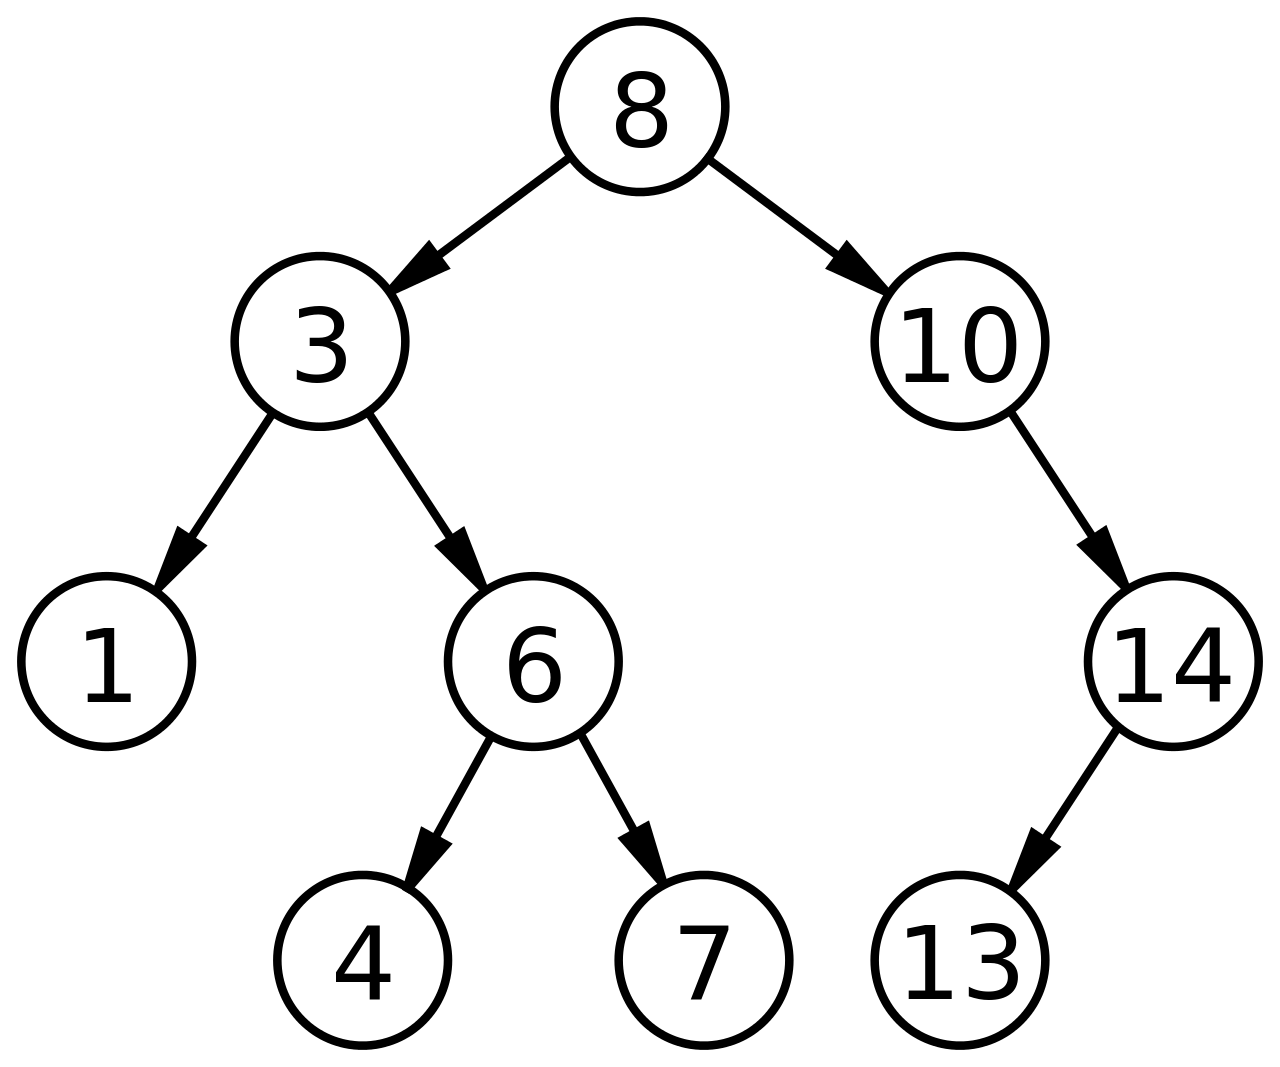
\includegraphics[scale=.1]{Del_Imgages/bst.png}
            \caption{Suppose delete 3, 1 or 14}
        \end{figure}
    \end{columns}
\end{frame}


\begin{frame}{Steps of Deletion}
    \begin{block}{Step 2}
        Fixup violations of Red-Black properties
    \end{block}
    \vspace{0.3cm}
    There are several cases that may occur during fixup operations.
\end{frame}

\begin{frame}{Steps of Deletion}
    \begin{block}{Case 1}
        If the node is \textbf{\textcolor{red}{Red}} which is to be deleted, we simply delete it.
    \end{block}
    \vspace{0.3cm}
    \begin{columns}
        \column[]{0.5\textwidth}
        \begin{figure}
            \centering
            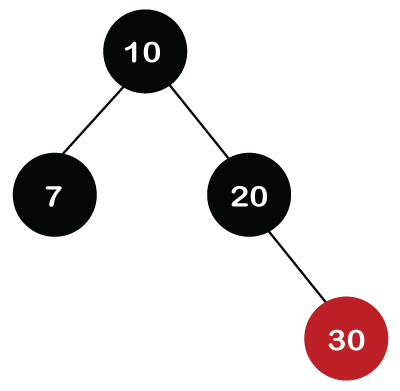
\includegraphics[scale=.3]{Del_Imgages/del1.1.png}
            \caption{Before deleting 30}
        \end{figure}
        \column[]{0.5\textwidth}
        \begin{figure}
            \centering
            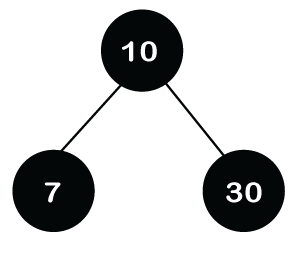
\includegraphics[scale=.3]{Del_Imgages/del1.2.png}
            \caption{After deleting 30}
        \end{figure}
    \end{columns}
\end{frame}

\begin{frame}{Steps of Deletion}
    \begin{block}{Case 2}
        If the node is a double black, just remove the double black (double black occurs when the node to be deleted is a black colored leaf node, as it adds up the NULL nodes which are considered black colored nodes too)
    \end{block}
\end{frame}

\begin{frame}{Steps of Deletion}
    \begin{block}{Case 3}
        If the double black's sibling node is also a black node and its child nodes are also black in color, follow the steps below:
        \vspace{0.3cm}
        \begin{itemize}
            \item Remove double black
            \item Recolor its parent to black (if the parent is a red node, it      becomes black; if the parent is already a black node, it            becomes double black)
            \item Recolor the parent's sibling with red
            \item If double black node still exists, we apply other cases.
        \end{itemize}
    \end{block}
\end{frame}

\begin{frame}{Steps of Deletion}
    \begin{block}{Case 4}
        If the double black node's sibling is red, we perform the following steps:
        \vspace{0.3cm}
        \begin{itemize}
            \item Swap the colors of the parent node and the parent's sibling       node.
            \item Rotate parent node in the double black's direction
            \item Reapply other cases that are suitable.
        \end{itemize}
    \end{block}
\end{frame}

\begin{frame}{Steps of Deletion}
    \begin{block}{Case 5}
        If the double black's sibling is a black node but the sibling's child node that is closest to the double black is red, follows the steps below:
        \vspace{0.3cm}
        \begin{itemize}
            \item Swap the colors of double black's sibling and the sibling's child in          question
            \item Rotate the sibling node is the opposite direction of double black (i.e. if    the double black is a right child apply left rotations and vice versa)
            \item Apply case 6.
        \end{itemize}
    \end{block}
\end{frame}

\begin{frame}{Steps of Deletion}
    \begin{block}{Case 6}
        If the double black's sibling is a black node but the sibling's child node that is farther to the double black is red, follows the steps below:
        \vspace{0.3cm}
        \begin{itemize}
            \item Swap the colors of double black's parent and sibling nodes
            \item Rotate the parent in double black's direction (i.e. if the double black is    a right    child apply right rotations and vice versa)
            \item Remove double black
            \item Change the color of red child node to black.
        \end{itemize}
    \end{block}
\end{frame}

\begin{frame}{Deletion Example}
    \begin{block}{Delete few elements}
        Delete 4
    \end{block}
    \begin{center}
        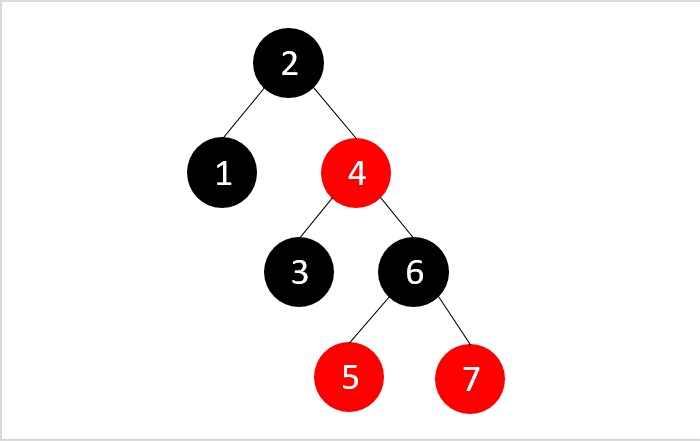
\includegraphics[scale=.7]{Del_Imgages/del_ex1.jpg} \\
    \end{center}
\end{frame}

\begin{frame}{Deletion Example}
    \begin{block}{Delete few elements}
        Delete 4
    \end{block}
    \begin{center}
        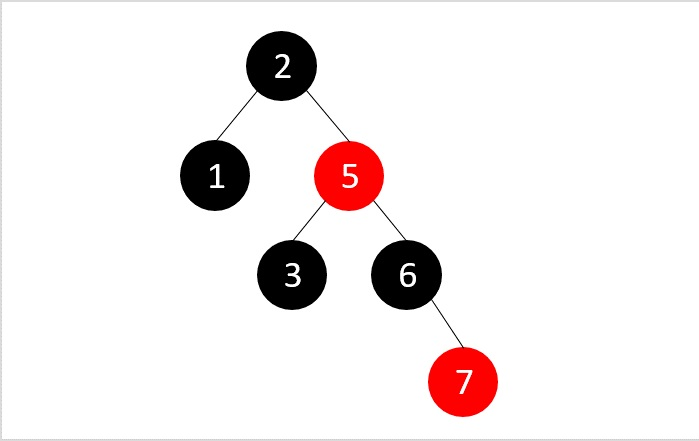
\includegraphics[scale=.7]{Del_Imgages/del_ex2.jpg} \\
    \end{center}
\end{frame}

\begin{frame}{Deletion Example}
    \begin{block}{Delete few elements}
        Delete 5
    \end{block}
    \begin{center}
        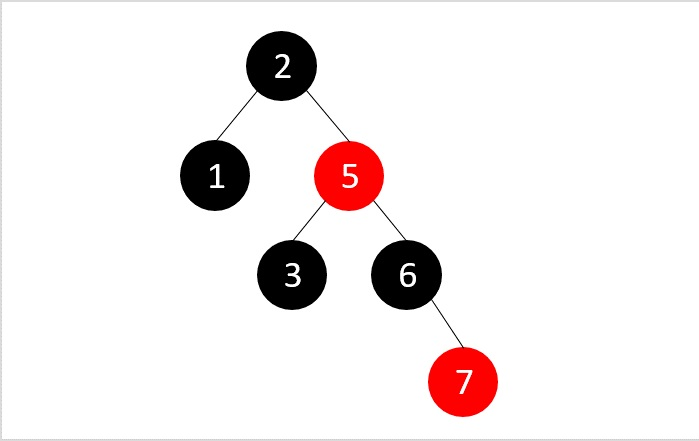
\includegraphics[scale=.7]{Del_Imgages/del_ex2.jpg} \\
    \end{center}
\end{frame}

\begin{frame}{Deletion Example}
    \begin{block}{Delete few elements}
        Delete 5
    \end{block}
    \begin{center}
        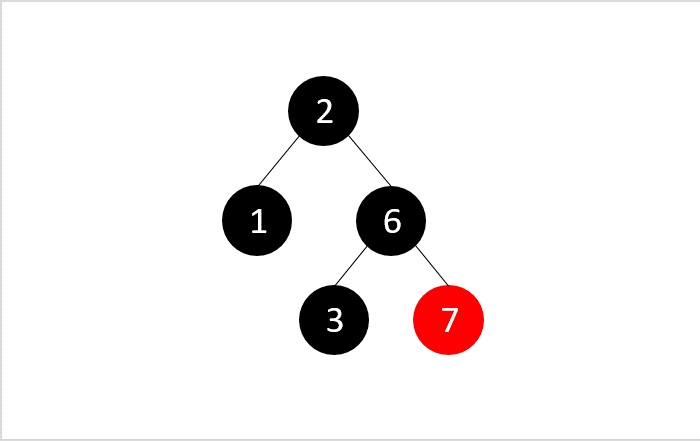
\includegraphics[scale=.7]{Del_Imgages/del_ex3.jpg} \\
    \end{center}
\end{frame}

\begin{frame}{Deletion Example}
    \begin{block}{Delete few elements}
        Delete 5
    \end{block}
    \begin{center}
        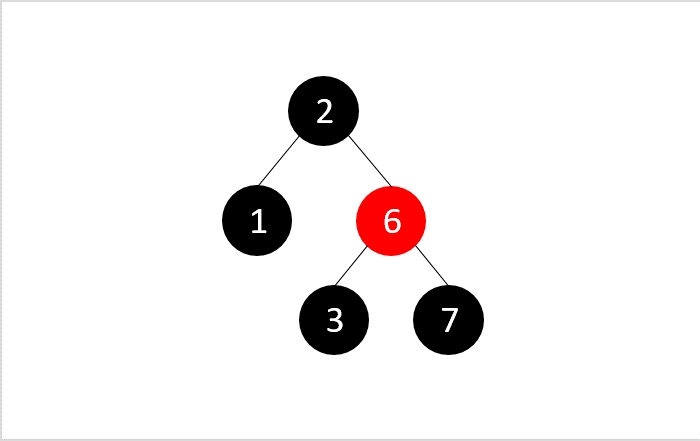
\includegraphics[scale=.7]{Del_Imgages/del_ex4.jpg} \\
    \end{center}
\end{frame}

\begin{frame}{Deletion Example}
    \begin{block}{Delete few elements}
        Delete 3
    \end{block}
    \begin{center}
        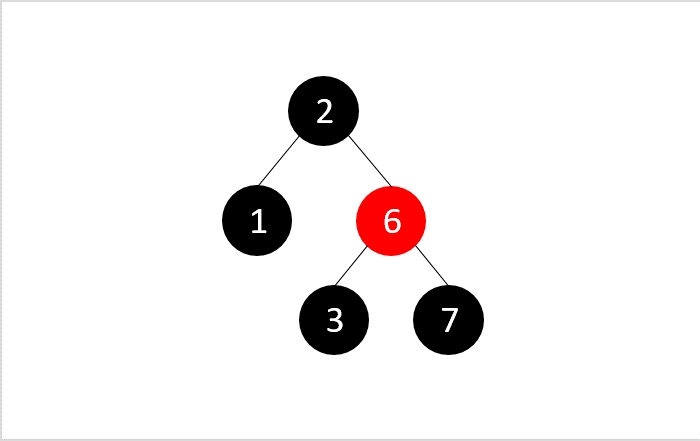
\includegraphics[scale=.7]{Del_Imgages/del_ex4.jpg} \\
    \end{center}
\end{frame}

\begin{frame}{Deletion Example}
    \begin{block}{Delete few elements}
        Delete 3
    \end{block}
    \begin{center}
        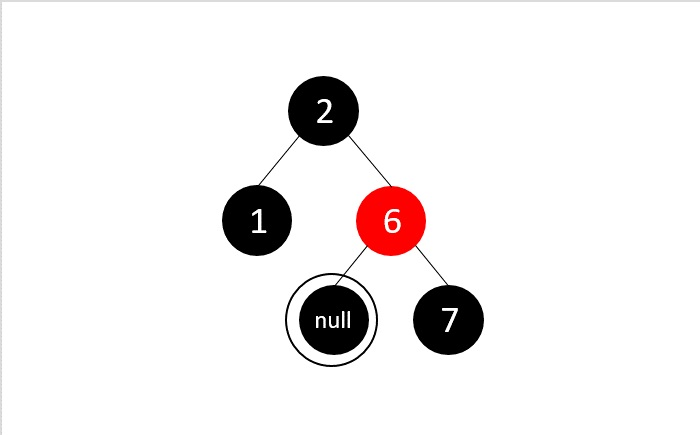
\includegraphics[scale=.7]{Del_Imgages/del_ex5.jpg} \\
    \end{center}
\end{frame}

\begin{frame}{Deletion Example}
    \begin{block}{Delete few elements}
        Delete 3
    \end{block}
    \begin{center}
        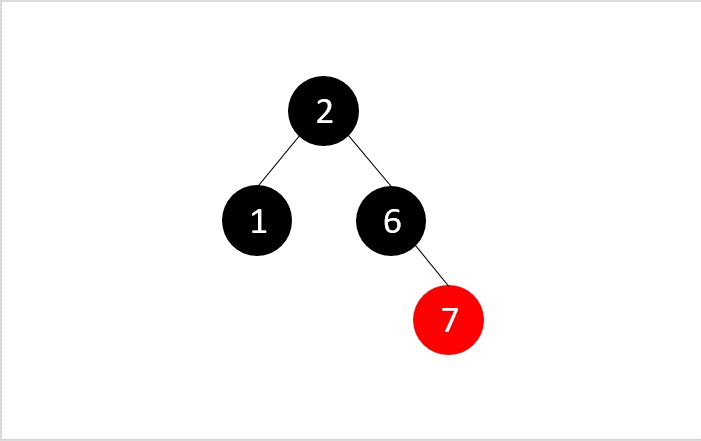
\includegraphics[scale=.7]{Del_Imgages/del_ex6.jpg} \\
    \end{center}
\end{frame}



\section{Application}
\begin{frame}{Red-Black Tree}
    \begin{center}
        {\Huge\textbf{\textcolor{blue}{Real-Life Use Cases}}}
    \end{center}
\end{frame}


\begin{frame}{Red-Black Trees: Real-Life Use Cases}
    \begin{block}{File Systems}
        Red-Black Trees are crucial for organizing files efficiently in file systems.
    \end{block}
    \vspace{0.3cm}
    \begin{center}
    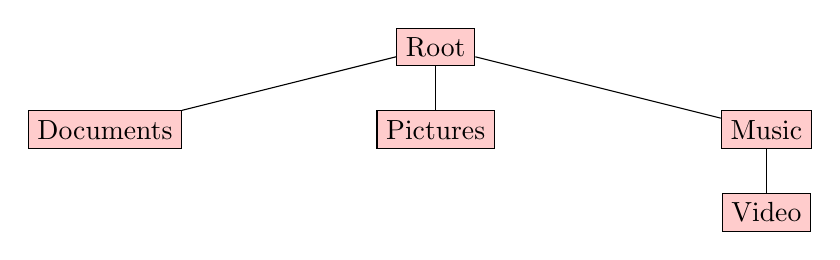
\begin{tikzpicture}[scale=0.7,level/.style={sibling distance=60mm/#1}]
    \tikzstyle{every node}=[rectangle,draw,fill=red!20,align=center]
    \node {Root}
      child {node {Documents}}
      child {node {Pictures}}
      child {node {Music}
        child{node{Video}}
      };
    \end{tikzpicture}
    \end{center}
\end{frame}


\begin{frame}{Balanced Trees: Real-Life Use Cases}
    \begin{block}{Database Indexing}
        Balanced trees enable quick retrieval of records in databases based on keys.
    \end{block}
    \vspace{0.3cm}
    \begin{center}
    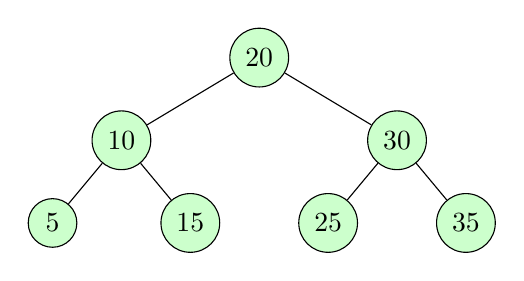
\begin{tikzpicture}[scale=0.7,level/.style={sibling distance=50mm/#1}]
    \tikzstyle{every node}=[circle,draw,fill=green!20]
    \node {20}
      child {node {10}
        child {node {5}}
        child {node {15}}
      }
      child {node {30}
        child {node {25}}
        child {node {35}}
      };
    \end{tikzpicture}
    \end{center}
\end{frame}

\begin{frame}{Balanced Trees: Real-Life Use Cases}
    \begin{block}{Symbol Tables in Compilers}
        Balanced trees are used to implement symbol tables for quick lookup of identifiers in compilers.
    \end{block}
    \vspace{0.3cm}
    \begin{center}
    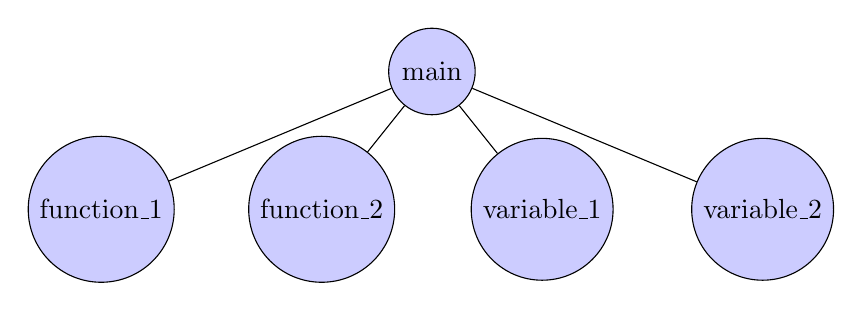
\begin{tikzpicture}[scale=0.7,level/.style={sibling distance=30mm/#1}]
    \tikzstyle{every node}=[circle,draw,fill=blue!20]
    \node {main}
      child[xshift=-1.5cm, yshift = -1cm] {node {function\_1}}
      child[xshift=-0.5cm , yshift = -1cm] {node {function\_2}}
      child[xshift=0.5cm, yshift = -1cm] {node {variable\_1}}
      child[xshift=1.5cm, yshift = -1cm] {node {variable\_2}};
    \end{tikzpicture}
    \end{center}
\end{frame}

\section*{The End}
\begin{frame}
    
\includegraphics[scale=0.455]{The_End.jpg}
\end{frame}



\end{document}